%------------------------------------------------------------------------------
% Template dos artigos da Revista LUPS
%------------------------------------------------------------------------------

\documentclass[12pt,article,compsoc]{IEEEtran}

%\usepackage[latin1]{inputenc}
\usepackage[utf8]{inputenc}

\usepackage[brazilian]{babel}
\usepackage[dvips]{graphicx}
\usepackage{epsfig}
\usepackage{amsfonts, color}
\usepackage{subfigure}
\usepackage{eurosym}
\usepackage[T1]{fontenc} 
\usepackage{ae}
\usepackage{cite}
\usepackage{amsthm}
\usepackage{hyperref}
\usepackage{booktabs}
\usepackage{scalefnt}

\newtheorem{definicao}{Definição}

%------------------------------------------------------------------------------

\begin{document}

%------------------------------------------------------------------------------
%%%%%%%%%%%%%%%%%%%%%%%%%%%%%%%%%%%%%%%%%%%%%%%%%%%%%%%%%%%%%%%%%%%%%%%%%%%%%%%
% Estas informações devem ser alteradas pelo editor da revista
\pubid{LABORATORY OF UBIQUITOUS AND PARALLEL SYSTEMS~\copyright~LUPS} 
\renewcommand{\leftmark}{REVISTA~LUPS,~VOL.~2, NO.~1,~NOVEMBRO~2019}
%%%%%%%%%%%%%%%%%%%%%%%%%%%%%%%%%%%%%%%%%%%%%%%%%%%%%%%%%%%%%%%%%%%%%%%%%%%%%%%
%------------------------------------------------------------------------------

% Título e autores do artigo

\title{Soluções voltadas para o gerenciamento de energia em Smart Homes}

\author{Maicon Robe Ferreira, UFPel; Guilherme Bayer Schneider, UFPel%

\IEEEcompsocitemizethanks{\IEEEcompsocthanksitem \textbf{Maicon Robe Ferreira}: Programa de Pós-Graduação em Computação,  Universidade Federal de Pelotas - UFPel, Centro de Desenvolvimento Tecnológigo - CDTec.
% Para uma quebra de linha, deve-se utilizar o \protect antes do \\, caso contrário vai dar erro.
\protect\\ E-mail: robemaicon@outlook.com}

% No caso de mais autores, basta repetir:
\IEEEcompsocitemizethanks{\IEEEcompsocthanksitem \textbf{Guilherme Bayer Schneider}: Programa de Pós-Graduação em Computação,  Universidade Federal de Pelotas - UFPel, Centro de Desenvolvimento Tecnológigo - CDTec. \protect\\ E-mail: guibayer2@gmail.com}
}

%------------------------------------------------------------------------------

\IEEEcompsoctitleabstractindextext{%
\begin{abstract}
Colocar o resumo
\end{abstract}

\begin{IEEEkeywords}
Palavra-chave 1, Palavra-chave 2, Palavra-chave 3, Palavra-chave 4.
\end{IEEEkeywords}}

\maketitle

%------------------------------------------------------------------------------

\section{Introdução}\label{sec:introducao}

\IEEEPARstart{S}{}mart Homes 

O último parágrafo da Introdução costuma ser dedicado a apresentar a estrutura do artigo. Neste parágrafo é feita uma breve descrição da intenção de cada seção.

%------------------------------------------------------------------------------

\section{Gerenciamento de Energia}\label{sec:gerenciamentoDeEnergia}

Colocar texto.

%------------------------------------------------------------------------------

\subsection{Energias Renováveis}

Colocar texto.

%------------------------------------------------------------------------------

\subsubsection{Energia Foto Voltaíca}

Colocar texto 

%------------------------------------------------------------------------------


\subsubsection{Energia Eólica}

Colocar texto 

%------------------------------------------------------------------------------

\subsection{Sistemas de Armazenamento de Energia}

Colocar texto.

%------------------------------------------------------------------------------

\subsection{Veículos Elétricos}

Colocar texto.

%------------------------------------------------------------------------------

\subsection{Programas de Resposta da Demanda}

Colocar texto.

%------------------------------------------------------------------------------

\section{Smart Home}\label{sec:smartHome}

Casa inteligente (\emph{Smart Home}) é um conceito que visa determinar que uma casa pode ser administrada com o auxílio de interfaces de internet das coisas (\emph{Internet of Things} - IoT), sejam elas para tomarem decisões autônomas quanto determinadas diretamente pelo usuário. 


As tecnologias de uma casa inteligente compreendem sensores, monitores, interfaces, dispositivos e dispositivos conectados em rede para permitir a automação, bem como o controle localizado e remoto do ambiente doméstico \cite{cook2012smart}. Aparelhos e dispositivos controláveis incluem sistemas de aquecimento e água quente, iluminação, janelas, cortinas, portas de garagem, geladeiras, TVs e máquinas de lavar \cite{robles2010applications}.

Sensores e monitores detectam fatores ambientes, incluindo temperatura, luz, movimento e umidade. A funcionalidade de controle é fornecida pelo software em dispositivos de computação (\emph{smartphones}, tablets, computadores) ou por meio de interfaces de hardware dedicadas (controles montados na parede). A conexão destes dispositivos pode ser cabeada ou sem fio. Essa diversidade traz diversas possibilidades de configuração e utilização de diferentes tecnologias nos ambientes de casas inteligentes. Essa grande diversidade é denominada \emph{"smartness"} \cite{harper2006inside}.

Em \cite{smartHomeDef} é apresentada uma definição de casa inteligente: 

\begin{definicao}
“Uma casa inteligente é uma casa que incorpora sistemas avançados de automação para fornecer aos habitantes monitoramento e controle sofisticados sobre as funções do edifício. Por exemplo, uma casa inteligente pode controlar as operações de iluminação, temperatura, multimídia, segurança, janelas e portas, além de muitas outras funções.”
\end{definicao}



%------------------------------------------------------------------------------

\subsection{Smart Grid}\label{sec:smartGrid}


Espera-se que o futuro sistema de energia faça uso extensivo das modernas tecnologias de informação e comunicação para apoiar um sistema de energia elétrica flexível, seguro e econômico. Em busca dessa eficiência diversos conceitos foram desenvolvidos, um deles é denominado Redes Inteligentes (\emph{Smart Grid}). Uma rede inteligente é capaz de controlar redes ativas de forma inteligente para facilitar a integração de energia renovável no sistema de energia~\cite{smartGridDef}.

Em \cite{smartGridDef2} a Associação de Redes de Energia (\emph{ Energy Networks Association - ENA}) define uma rede inteligente:

\begin{definicao}

A Rede Inteligente é tudo, desde a geração até a automação residencial, com um medidor inteligente sendo um elemento importante, com todos os equipamentos de rede, tecnologia de comunicação e processos entre os quais contribuem para uma grade inteligente e eficiente.

Uma rede totalmente inteligente do futuro permitirá que os aparelhos domésticos se comuniquem com o medidor inteligente e as redes para garantir o uso eficiente da infraestrutura, resposta à demanda e gerenciamento de energia. Tudo isso é fundamental para aproveitar ao máximo as energias renováveis intermitentes e manter as luzes acesas em um futuro acessível de energia de baixo carbono.

\end{definicao}


Simplificando, a rede tradicional só pode transmitir ou distribuir energia elétrica já rede inteligente é capaz de armazenar, comunicar e tomar decisões. Uma Rede Inteligente transforma a rede tradicional em uma que funcione de maneira mais cooperativa, responsiva e orgânica \cite{smartGridIntroduction}.

Na tabela \ref{tab:tabelaComparativa} é feita uma comparação das características de uma rede tradicional com as de uma rede inteligente.

\begin{table}[]
\centering
\scalefont{0.67}
\label{tab:tabelaComparativa}
\begin{tabular}{|c||c|c|}
\hline
 & Rede Tradicional & Rede Inteligente \\ \hline
Comunicação & Não ou só de ida & Bidirecional \\ \hline
\begin{tabular}[c]{@{}c@{}}Interação com \\ o usuário\end{tabular} & Raramente & Muita \\ \hline
Tipo de Instrumento & Elétrico & Numérico \\ \hline
Operação e Gerência & \begin{tabular}[c]{@{}c@{}}Calibração de\\ dispositivo artificial\end{tabular} & \begin{tabular}[c]{@{}c@{}}Monitoramento\\  Remoto\end{tabular} \\ \hline
Controle de Fluxo & Limitado & Universal \\ \hline
Confiabilidade & \begin{tabular}[c]{@{}c@{}}Tendem a mau \\ funcionamento e \\ interrupção de energia\end{tabular} & Proteção adaptativa \\ \hline
Recuperação & Artificial & Auto-cura \\ \hline
\end{tabular}
\caption{Comparação entre a Rede Tradicional e a Rede Inteligente}
\end{table}



%------------------------------------------------------------------------------

\subsection{Smart Plug}\label{sec:smartPlug}

Colocar texto

%------------------------------------------------------------------------------

\subsection{Smart Appliance}

Colocar texto.

%--------------------------------------------------------------

\subsubsection{Eletrodomésticos}

Colocar texto.

%------------------------------------------------------------------------------

\subsubsection{Assistentes virtuais}

Colocar texto.

%------------------------------------------------------------------------------

\subsubsection{Sistemas de segurança}

Colocar texto.

%------------------------------------------------------------------------------

\section{Técnicas de gerenciamento em Smart Homes}\label{sec:tecnicasDeGerenciamento}

Colocar texto.

%------------------------------------------------------------------------------

\section{Levantamento Bibliográfico}\label{sec:levantamentoBibliografico}

Colocar texto.

%------------------------------------------------------------------------------

\section{Trabalhos relacionados}\label{sec:relacionados}

Colocar texto.

%------------------------------------------------------------------------------

\subsection{Trabalho 1}

Colocar texto.

%------------------------------------------------------------------------------

\subsection{Trabalho 2}

Colocar texto.

%------------------------------------------------------------------------------

\subsection{Trabalho 3}

Colocar texto.

%------------------------------------------------------------------------------

\section{Considerações Finais}\label{sec:consideracoesFinais}

Colocar texto.

%------------------------------------------------------------------------------

\bibliographystyle{unsrt}
\bibliography{BIBFile}

%------------------------------------------------------------------------------
%Biografia dos autores

\begin{IEEEbiography}[{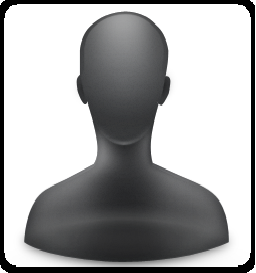
\includegraphics[width=1in, height=1.25in, clip, keepaspectratio]{imagens/fotodoautor.png}}]{Nome do Autor 1}
Colocar uma biografia do Autor 1 aqui, similar a apresentação do Currículo Lattes. Exemplo: Mestrando do Programa de Pós-Graduação em Computação da Universidade Federal de Pelotas, na linha de pesquisa Sistemas Paralelos e Distribuídos. Também é pós-graduando \textit{Lato Sensu} em (...) pela Universidade (...) . Possui Bacharelado (2011) em Ciência da Computação pela Universidade (...). Tem experiência na área de Ciência da Computação, com ênfase nas áreas de (...).
Quanto a foto, não deve ser de corpo inteiro (deve ser similar ao avatar de exemplo) e convertida em escala de cinza.
\end{IEEEbiography}


\begin{IEEEbiography}[{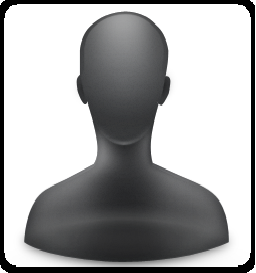
\includegraphics[width=1in, height=1.25in, clip, keepaspectratio]{imagens/fotodoautor.png}}]{Nome do Autor 2}
Colocar uma biografia do Autor 2 aqui, similar a apresentação do Currículo Lattes. Exemplo: Mestrando do Programa de Pós-Graduação em Computação da Universidade Federal de Pelotas, na linha de pesquisa Sistemas Paralelos e Distribuídos. Também é pós-graduando \textit{Lato Sensu} em (...) pela Universidade (...) . Possui Bacharelado (2011) em Ciência da Computação pela Universidade (...). Tem experiência na área de Ciência da Computação, com ênfase nas áreas de (...).
Quanto a foto, não deve ser de corpo inteiro (deve ser similar ao avatar de exemplo) e convertida em escala de cinza.
\end{IEEEbiography}

\end{document}


